\newpage
\section{Sprint 2}
\label{sec:sprint2}

Siguiendo la planificación inicial detallada en la sección \ref{sec:planificacion-inicial}, el segundo sprint se enfoca exclusivamente en el desarrollo de la \textbf{aplicación móvil}. El objetivo principal es sentar las bases de la aplicación cliente, creando una estructura de proyecto robusta, implementando los módulos nativos necesarios para funcionalidades clave y desarrollando una primera versión de la interfaz de usuario.

El entregable al final de este sprint será una aplicación de galería básica que pueda solicitar los permisos necesarios, acceder a las fotos y vídeos del dispositivo y mostrarlos en una interfaz de usuario funcional. Aún no se implementarán las funcionalidades de sincronización con el servidor, ya que el foco está en la arquitectura del cliente y su interacción con el sistema operativo móvil.

La velocidad del equipo del sprint anterior se utilizará como referencia, pero al cambiar completamente el contexto de desarrollo (de backend a móvil), se asume una incertidumbre similar a la del primer sprint. La selección de historias se ha realizado buscando un equilibrio entre la creación de la estructura fundamental y la implementación de una primera funcionalidad visible.

\subsection{Historias de usuario}
A continuación, se presentan las historias de usuario y técnicas seleccionadas para este sprint, priorizando la creación del esqueleto de la aplicación móvil y la interacción con el sistema nativo.

Las historias seleccionadas son las siguientes:
\begin{itemize}
    \item HU20: Ver archivos subidos (adaptada a "Ver archivos locales") - 5 PH
    \item HU24: Inicio y cierre de sesión - 5 PH
    \item HU25: Gestión de permisos - 3 PH
    \item HT23: Acceso a la galería - 5 PH
    \item HT24: Comunicación con API - 5 PH
    \item HT29: Pruebas unitarias - 5 PH (parcial)
    \item HT31: Gestión de tokens - 3 PH
    \item HT36: UI responsive - 3 PH
\end{itemize}

La suma total de las historias seleccionadas es de \textbf{34 puntos de historia (PH)}. Aunque el número de puntos es menor que en el sprint anterior, la complejidad de configurar un nuevo entorno de desarrollo móvil y la implementación de módulos nativos justifica una carga de trabajo similar.

Además, se estima una carga extra a la hora de implementar los módulos nativos y la integración con Lynx.js, lo que puede hacer que el esfuerzo real sea comparable al del primer sprint.

\textbf{Descomposición en tareas de desarrollo}

% HU20: Ver archivos subidos (adaptada)
\begin{table}[H]
    \begin{center}
        \begin{tabularx}{\textwidth}{|l|X|l|}
            \hline
            \textbf{Identificador HU20} &
            \textbf{Como usuario, quiero ver una lista o galería de los archivos que ya están en mi dispositivo} &
            \textbf{Estimación: 5 PH}\\
            \hline
            \multicolumn{3}{|p{\textwidth}|}{
                \begin{minipage}{\textwidth}
                    \centering
                    \vspace{0.5em}
                    \begin{tabular}{|l|p{8cm}|r|}
                        \hline
                        \textbf{Identificador} & \textbf{Título de la tarea de desarrollo} & \makecell{\textbf{Estimación}\\\textbf{(h)}} \\
                        \hline
                        Tarea 20-1 & Crear el componente de la pantalla principal (galería) & 4.5 \\
                        \hline
                        Tarea 20-2 & Implementar un componente para previsualizar cada imagen (thumbnail) & 4 \\
                        \hline
                        Tarea 20-3 & Diseñar y maquetar una cuadrícula (grid) para mostrar las imágenes & 2 \\
                        \hline
                        Tarea 20-4 & Integrar la lógica para obtener las imágenes del dispositivo (depende de HT23) & 3 \\
                        \hline
                    \end{tabular}
                    \vspace{0.5em}
                \end{minipage}
            } \\
            \hline
            \multicolumn{3}{|p{\textwidth}|}{
                \textbf{Pruebas de aceptación:}
                \begin{itemize}
                    \item Al abrir la app (tras iniciar sesión), se muestra una galería con las imágenes del móvil.
                    \item Las imágenes se muestran en una cuadrícula ordenada.
                    \item La interfaz es fluida al desplazarse por la galería.
                \end{itemize}
            }\\
            \hline
            \multicolumn{3}{|p{\textwidth}|}{
                \textbf{Observaciones:}
                \begin{itemize}
                    \item La historia original era ``ver archivos subidos'', pero se adapta para este sprint a ``ver archivos locales'' como primer paso.
                    \item Inicialmente no se incluirá la carga de vídeos, solo imágenes.
                \end{itemize}
            }\\
            \hline
        \end{tabularx}
    \end{center}
\end{table}

% HU24: Inicio y cierre de sesión
\begin{table}[H]
    \begin{center}
        \begin{tabularx}{\textwidth}{|l|X|l|}
            \hline
            \textbf{Identificador HU24} &
            \textbf{Como usuario, quiero iniciar y cerrar sesión para proteger mis datos} &
            \textbf{Estimación: 5 PH}\\
            \hline
            \multicolumn{3}{|p{\textwidth}|}{
                \begin{minipage}{\textwidth}
                    \centering
                    \vspace{0.5em}
                    \begin{tabular}{|l|p{8cm}|r|}
                        \hline
                        \textbf{Identificador} & \textbf{Título de la tarea de desarrollo} & \makecell{\textbf{Estimación}\\\textbf{(h)}} \\
                        \hline
                        Tarea 24-1U & Diseñar y maquetar la pantalla de inicio de sesión & 2 \\
                        \hline
                        Tarea 24-2U & Implementar la lógica del formulario (usuario, contraseña) & 1.5 \\
                        \hline
                        Tarea 24-3U & Integrar la llamada al endpoint de login del servidor (depende de HT24) & 2 \\
                        \hline
                        Tarea 24-4U & Implementar la navegación: si el login es exitoso, ir a la galería & 1 \\
                        \hline
                        Tarea 24-5U & Añadir un botón para cerrar sesión que borre el token (depende de HT31) & 1 \\
                        \hline
                    \end{tabular}
                    \vspace{0.5em}
                \end{minipage}
            } \\
            \hline
            \multicolumn{3}{|p{\textwidth}|}{
                \textbf{Pruebas de aceptación:}
                \begin{itemize}
                    \item El usuario puede introducir sus credenciales y pulsar un botón para iniciar sesión.
                    \item Si las credenciales son válidas, se le redirige a la pantalla de la galería.
                    \item Si son inválidas, se muestra un mensaje de error.
                    \item Existe una opción para cerrar la sesión actual.
                \end{itemize}
            }\\
            \hline
            \multicolumn{3}{|p{\textwidth}|}{
                \textbf{Observaciones:}
                \begin{itemize}
                    \item Esta HU conecta el cliente con el backend desarrollado en el Sprint 1.
                \end{itemize}
            }\\
            \hline
        \end{tabularx}
    \end{center}
\end{table}

% HU25: Gestión de permisos
\begin{table}[H]
    \begin{center}
        \begin{tabularx}{\textwidth}{|l|X|l|}
            \hline
            \textbf{Identificador HU25} &
            \textbf{Como usuario, quiero que la app me pida permisos de acceso solo cuando sea necesario} &
            \textbf{Estimación: 3 PH}\\
            \hline
            \multicolumn{3}{|p{\textwidth}|}{
                \begin{minipage}{\textwidth}
                    \centering
                    \vspace{0.5em}
                    \begin{tabular}{|l|p{8cm}|r|}
                        \hline
                        \textbf{Identificador} & \textbf{Título de la tarea de desarrollo} & \makecell{\textbf{Estimación}\\\textbf{(h)}} \\
                        \hline
                        Tarea 25-1 & Implementar la lógica para verificar si los permisos ya han sido concedidos & 1 \\
                        \hline
                        Tarea 25-2 & Invocar el diálogo nativo de solicitud de permisos de lectura de almacenamiento & 1.5 \\
                        \hline
                        Tarea 25-3 & Gestionar la respuesta del usuario (permiso concedido o denegado) & 1.5 \\
                        \hline
                    \end{tabular}
                    \vspace{0.5em}
                \end{minipage}
            } \\
            \hline
            \multicolumn{3}{|p{\textwidth}|}{
                \textbf{Pruebas de aceptación:}
                \begin{itemize}
                    \item Al intentar acceder a la galería por primera vez, la app solicita permiso para leer el almacenamiento.
                    \item Si el usuario concede el permiso, la app muestra las imágenes.
                    \item Si el usuario deniega el permiso, la app muestra un mensaje informativo.
                \end{itemize}
            }\\
            \hline
            \multicolumn{3}{|p{\textwidth}|}{
                \textbf{Observaciones:}
                \begin{itemize}
                    \item Esta historia está ligada a la implementación del módulo nativo (HT23).
                \end{itemize}
            }\\
            \hline
        \end{tabularx}
    \end{center}
\end{table}

% HT23: Acceso a la galería
\begin{table}[H]
    \begin{center}
        \begin{tabularx}{\textwidth}{|l|X|l|}
            \hline
            \textbf{Identificador HT23} &
            \textbf{Implementar acceso seguro a la galería de fotos y vídeos} &
            \textbf{Estimación: 5 PH}\\
            \hline
            \multicolumn{3}{|p{\textwidth}|}{
                \begin{minipage}{\textwidth}
                    \centering
                    \vspace{0.5em}
                    \begin{tabular}{|l|p{8cm}|r|}
                        \hline
                        \textbf{Identificador} & \textbf{Título de la tarea de desarrollo} & \makecell{\textbf{Estimación}\\\textbf{(h)}} \\
                        \hline
                        Tarea 23-1 & Configurar el proyecto `Lynx Explorer' para añadir un módulo nativo en Android & 3 \\
                        \hline
                        Tarea 23-2 & Escribir el código nativo (Java/Kotlin) para consultar el `MediaStore' de Android & 3 \\
                        \hline
                        Tarea 23-3 & Crear el ``puente'' (bridge) para exponer la funcionalidad nativa a JavaScript & 2.5 \\
                        \hline
                        Tarea 23-4 & Implementar el método en JS que llama al módulo nativo para obtener las URIs de las imágenes & 2 \\
                        \hline
                    \end{tabular}
                    \vspace{0.5em}
                \end{minipage}
            } \\
            \hline
            \multicolumn{3}{|p{\textwidth}|}{
                \textbf{Pruebas de aceptación:}
                \begin{itemize}
                    \item El código JavaScript puede invocar una función que devuelve una lista de imágenes del dispositivo.
                    \item El módulo nativo gestiona correctamente los permisos y errores de acceso.
                    \item La app puede compilarse con el nuevo módulo nativo incluido.
                \end{itemize}
            }\\
            \hline
            \multicolumn{3}{|p{\textwidth}|}{
                \textbf{Observaciones:}
                \begin{itemize}
                    \item Esta es una de las tareas más complejas y críticas del sprint, ya que valida el uso de una de las características clave de Lynx.js.
                \end{itemize}
            }\\
            \hline
        \end{tabularx}
    \end{center}
\end{table}


% HT24: Comunicación con API
\begin{table}[H]
    \begin{center}
        \begin{tabularx}{\textwidth}{|l|X|l|}
            \hline
            \textbf{Identificador HT24} &
            \textbf{Integrar cliente HTTP que se comunique con el servidor} &
            \textbf{Estimación: 5 PH}\\
            \hline
            \multicolumn{3}{|p{\textwidth}|}{
                \begin{minipage}{\textwidth}
                    \centering
                    \vspace{0.5em}
                    \begin{tabular}{|l|p{8cm}|r|}
                        \hline
                        \textbf{Identificador} & \textbf{Título de la tarea de desarrollo} & \makecell{\textbf{Estimación}\\\textbf{(h)}} \\
                        \hline
                        Tarea 24-1 & Seleccionar e instalar una librería de cliente HTTP (ej. axios) & 0.5 \\
                        \hline
                        Tarea 24-2 & Crear una capa de servicio (service layer) para encapsular las llamadas a la API & 2 \\
                        \hline
                        Tarea 24-3 & Definir los \glspl{dto} para las peticiones y respuestas & 1.5 \\
                        \hline
                        Tarea 24-4 & Implementar la lógica para añadir el token JWT a las cabeceras de las peticiones & 1.5 \\
                        \hline
                    \end{tabular}
                    \vspace{0.5em}
                \end{minipage}
            } \\
            \hline
            \multicolumn{3}{|p{\textwidth}|}{
                \textbf{Pruebas de aceptación:}
                \begin{itemize}
                    \item La aplicación puede realizar una petición POST al endpoint de login.
                    \item Se puede configurar la URL base del servidor mediante variables de entorno (en sprints posteriores, esta url se descubrirá automáticamente en la red).
                    \item La capa de servicio maneja correctamente las respuestas exitosas y de error.
                \end{itemize}
            }\\
            \hline
            \multicolumn{3}{|p{\textwidth}|}{
                \textbf{Observaciones:}
                \begin{itemize}
                    \item La implementación seguirá los principios de la arquitectura limpia, aislando la infraestructura de red.
                \end{itemize}
            }\\
            \hline
        \end{tabularx}
    \end{center}
\end{table}

% HT29: Pruebas unitarias
\begin{table}[H]
    \begin{center}
        \begin{tabularx}{\textwidth}{|l|X|l|}
            \hline
            \textbf{Identificador HT29} &
            \textbf{Añadir pruebas unitarias y de integración a la lógica común en React / Lynx.js} &
            \textbf{Estimación: 5 PH (Parcial)}\\
            \hline
            \multicolumn{3}{|p{\textwidth}|}{
                \begin{minipage}{\textwidth}
                    \centering
                    \vspace{0.5em}
                    \begin{tabular}{|l|p{8cm}|r|}
                        \hline
                        \textbf{Identificador} & \textbf{Título de la tarea de desarrollo} & \makecell{\textbf{Estimación}\\\textbf{(h)}} \\
                        \hline
                        Tarea 29-1 & Configurar el entorno de pruebas (Jest) & 2 \\
                        \hline
                        Tarea 29-2 & Escribir pruebas para los servicios de la capa de aplicación (ej. servicio de autenticación) & 2.5 \\
                        \hline
                    \end{tabular}
                    \vspace{0.5em}
                \end{minipage}
            } \\
            \hline
            \multicolumn{3}{|p{\textwidth}|}{
                \textbf{Pruebas de aceptación:}
                \begin{itemize}
                    \item Se pueden ejecutar las pruebas desde la línea de comandos.
                    \item Los componentes visuales tienen pruebas que verifican su renderizado y comportamiento.
                    \item La lógica de negocio está cubierta por pruebas unitarias.
                    \item Las dependencias externas (API, módulos nativos) están mockeadas en las pruebas.
                \end{itemize}
            }\\
            \hline
            \multicolumn{3}{|p{\textwidth}|}{
                \textbf{Observaciones:}
                \begin{itemize}
                    \item Es una historia técnica de alta estimación porque establecer una buena base de pruebas desde el principio es fundamental para la mantenibilidad del proyecto.
                \end{itemize}
            }\\
            \hline
        \end{tabularx}
    \end{center}
\end{table}

% HT31: Gestión de tokens
\begin{table}[H]
    \begin{center}
        \begin{tabularx}{\textwidth}{|l|X|l|}
            \hline
            \textbf{Identificador HT31} &
            \textbf{Almacenar y renovar tokens de autenticación de forma segura} &
            \textbf{Estimación: 3 PH}\\
            \hline
            \multicolumn{3}{|p{\textwidth}|}{
                \begin{minipage}{\textwidth}
                    \centering
                    \vspace{0.5em}
                    \begin{tabular}{|l|p{8cm}|r|}
                        \hline
                        \textbf{Identificador} & \textbf{Título de la tarea de desarrollo} & \makecell{\textbf{Estimación}\\\textbf{(h)}} \\
                        \hline
                        Tarea 31-1 & Investigar y elegir una solución de almacenamiento seguro local (ej. AsyncStorage) & 1 \\
                        \hline
                        Tarea 31-2 & Crear un servicio para guardar, leer y eliminar el token JWT del almacenamiento & 2 \\
                        \hline
                        Tarea 31-3 & Integrar este servicio en el flujo de inicio y cierre de sesión & 1 \\
                        \hline
                    \end{tabular}
                    \vspace{0.5em}
                \end{minipage}
            } \\
            \hline
            \multicolumn{3}{|p{\textwidth}|}{
                \textbf{Pruebas de aceptación:}
                \begin{itemize}
                    \item Tras un inicio de sesión exitoso, el token JWT se guarda en el dispositivo.
                    \item Al cerrar la aplicación y volver a abrirla, el usuario sigue autenticado (se recupera el token).
                    \item Al cerrar sesión, el token se elimina del almacenamiento.
                \end{itemize}
            }\\
            \hline
        \end{tabularx}
    \end{center}
\end{table}

% HT36: UI responsive
\begin{table}[H]
    \begin{center}
        \begin{tabularx}{\textwidth}{|l|X|l|}
            \hline
            \textbf{Identificador HT36} &
            \textbf{Adaptar UI para distintos tamaños de pantalla (tablet, móvil)} &
            \textbf{Estimación: 3 PH}\\
            \hline
            \multicolumn{3}{|p{\textwidth}|}{
                \begin{minipage}{\textwidth}
                    \centering
                    \vspace{0.5em}
                    \begin{tabular}{|l|p{8cm}|r|}
                        \hline
                        \textbf{Identificador} & \textbf{Título de la tarea de desarrollo} & \makecell{\textbf{Estimación}\\\textbf{(h)}} \\
                        \hline
                        Tarea 36-1 & Implementar una estrategia de diseño adaptable & 2 \\
                        \hline
                        Tarea 36-2 & Probar y ajustar la UI de la galería y el login en emuladores de tablet y móvil & 2 \\
                        \hline
                    \end{tabular}
                    \vspace{0.5em}
                \end{minipage}
            } \\
            \hline
            \multicolumn{3}{|p{\textwidth}|}{
                \textbf{Pruebas de aceptación:}
                \begin{itemize}
                    \item La pantalla de login se ve correctamente tanto en un móvil de tamaño estándar como en una tablet.
                    \item La cuadrícula de la galería adapta el número de columnas según el ancho de la pantalla.
                \end{itemize}
            }\\
            \hline
        \end{tabularx}
    \end{center}
\end{table}

\paragraph{Resumen de estimación de tareas}

El total de horas estimadas para las tareas de desarrollo del Sprint 2 es de \textbf{53.5 horas}, cifra que se acerca a la capacidad teórica del sprint (56 horas). La distribución es la siguiente:

\begin{itemize}
    \item HU20 (Ver archivos locales): 13.5 horas
    \item HU24 (Inicio y cierre de sesión): 7.5 horas
    \item HU25 (Gestión de permisos): 4 horas
    \item HT23 (Acceso a la galería): 10.5 horas
    \item HT24 (Comunicación con API): 5.5 horas
    \item HT29 (Pruebas unitarias): 4.5 horas
    \item HT31 (Gestión de tokens): 4 horas
    \item HT36 (UI responsive): 4 horas
\end{itemize}

Se observa que historias técnicas como HT23 (módulo nativo) y HU20 (archivos locales) consumen una parte significativa del tiempo. Esto se debe a la complejidad de implementar módulos nativos y establecer una base sólida para la aplicación móvil. El desarrollo de los módulos nativos se realiza en Kotlin/Java, entorno en el que el equipo no tiene ninguna experiencia previa.

\subsection{Diagrama de Gantt}
A la hora de realizar las tareas se ha priorizado la visualización de una galería funcional en la aplicación. Una vez que se tenga una galería funcional, se implementarán las funcionalidades que tienen que ver con la comunicación con la API. El acceso a la galería (HT23) es una tarea crítica que debe completarse antes de poder implementar la visualización de archivos locales (HU20), es por ello que las tareas relacionadas con la historia técnica van antes que las de la historia de usuario.

\begin{figure}[H]
    \begin{center}
        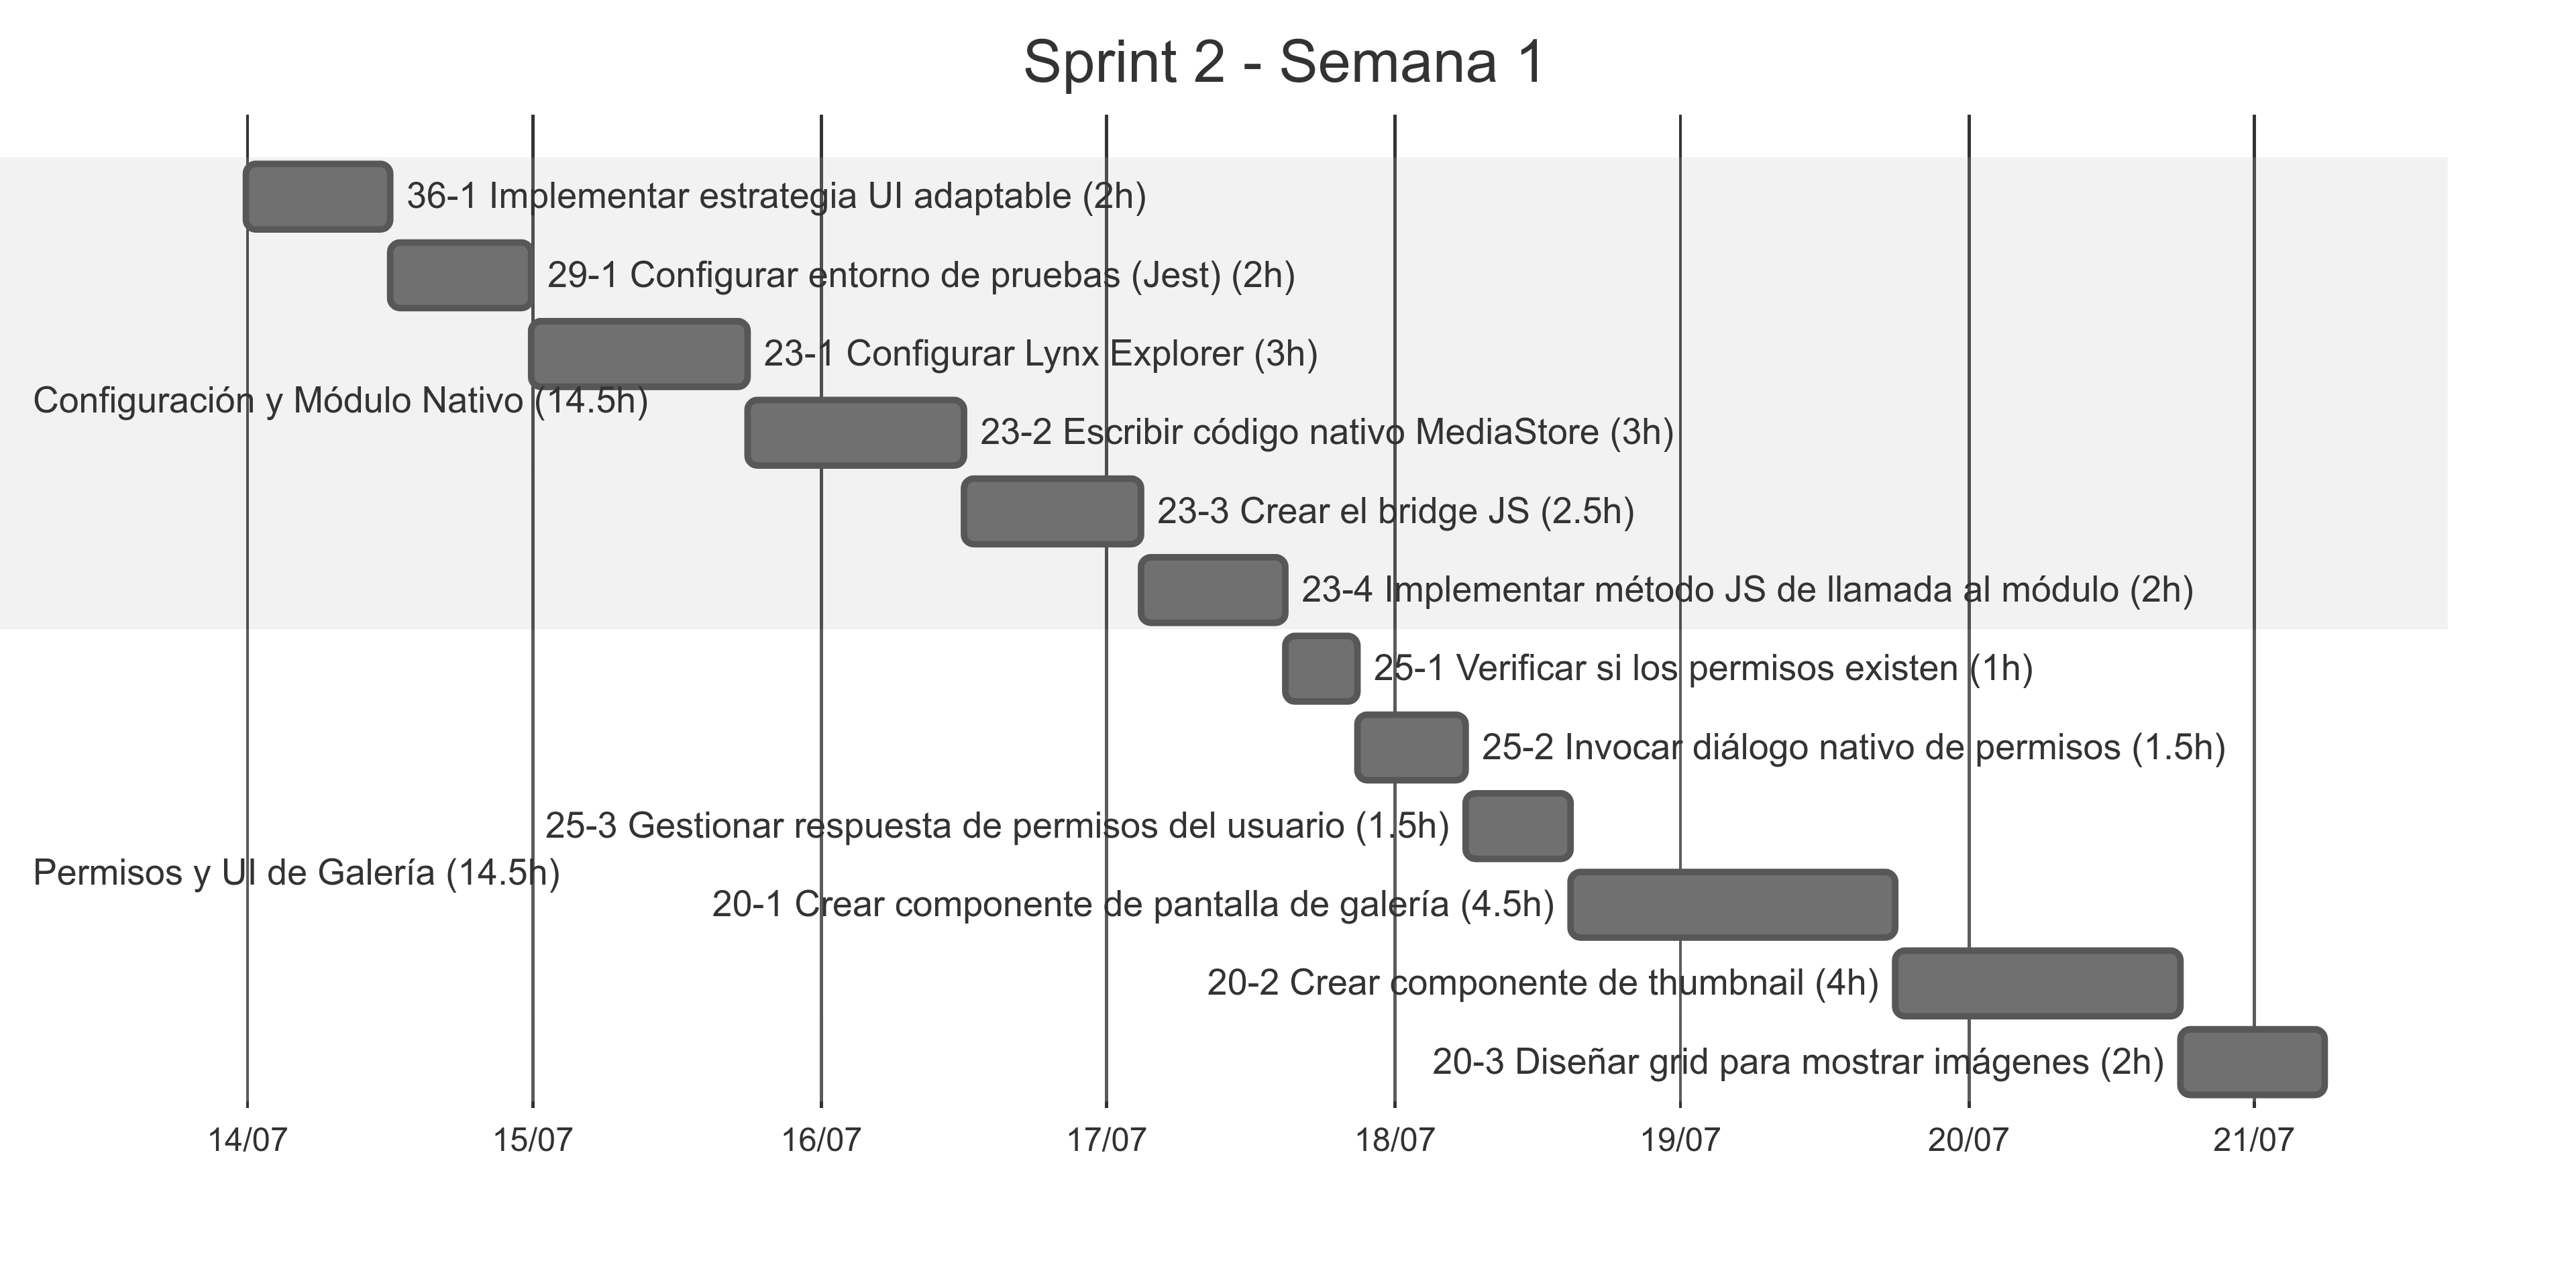
\includegraphics[width=0.8\textwidth]{assets/sprint2/week1-gantt.png}
    \end{center}
    \caption{Diagrama de Gantt de las tareas de la primera semana del sprint 2}\label{fig:gantt-sprint2-week1}
\end{figure}

\begin{figure}[H]
    \begin{center}
        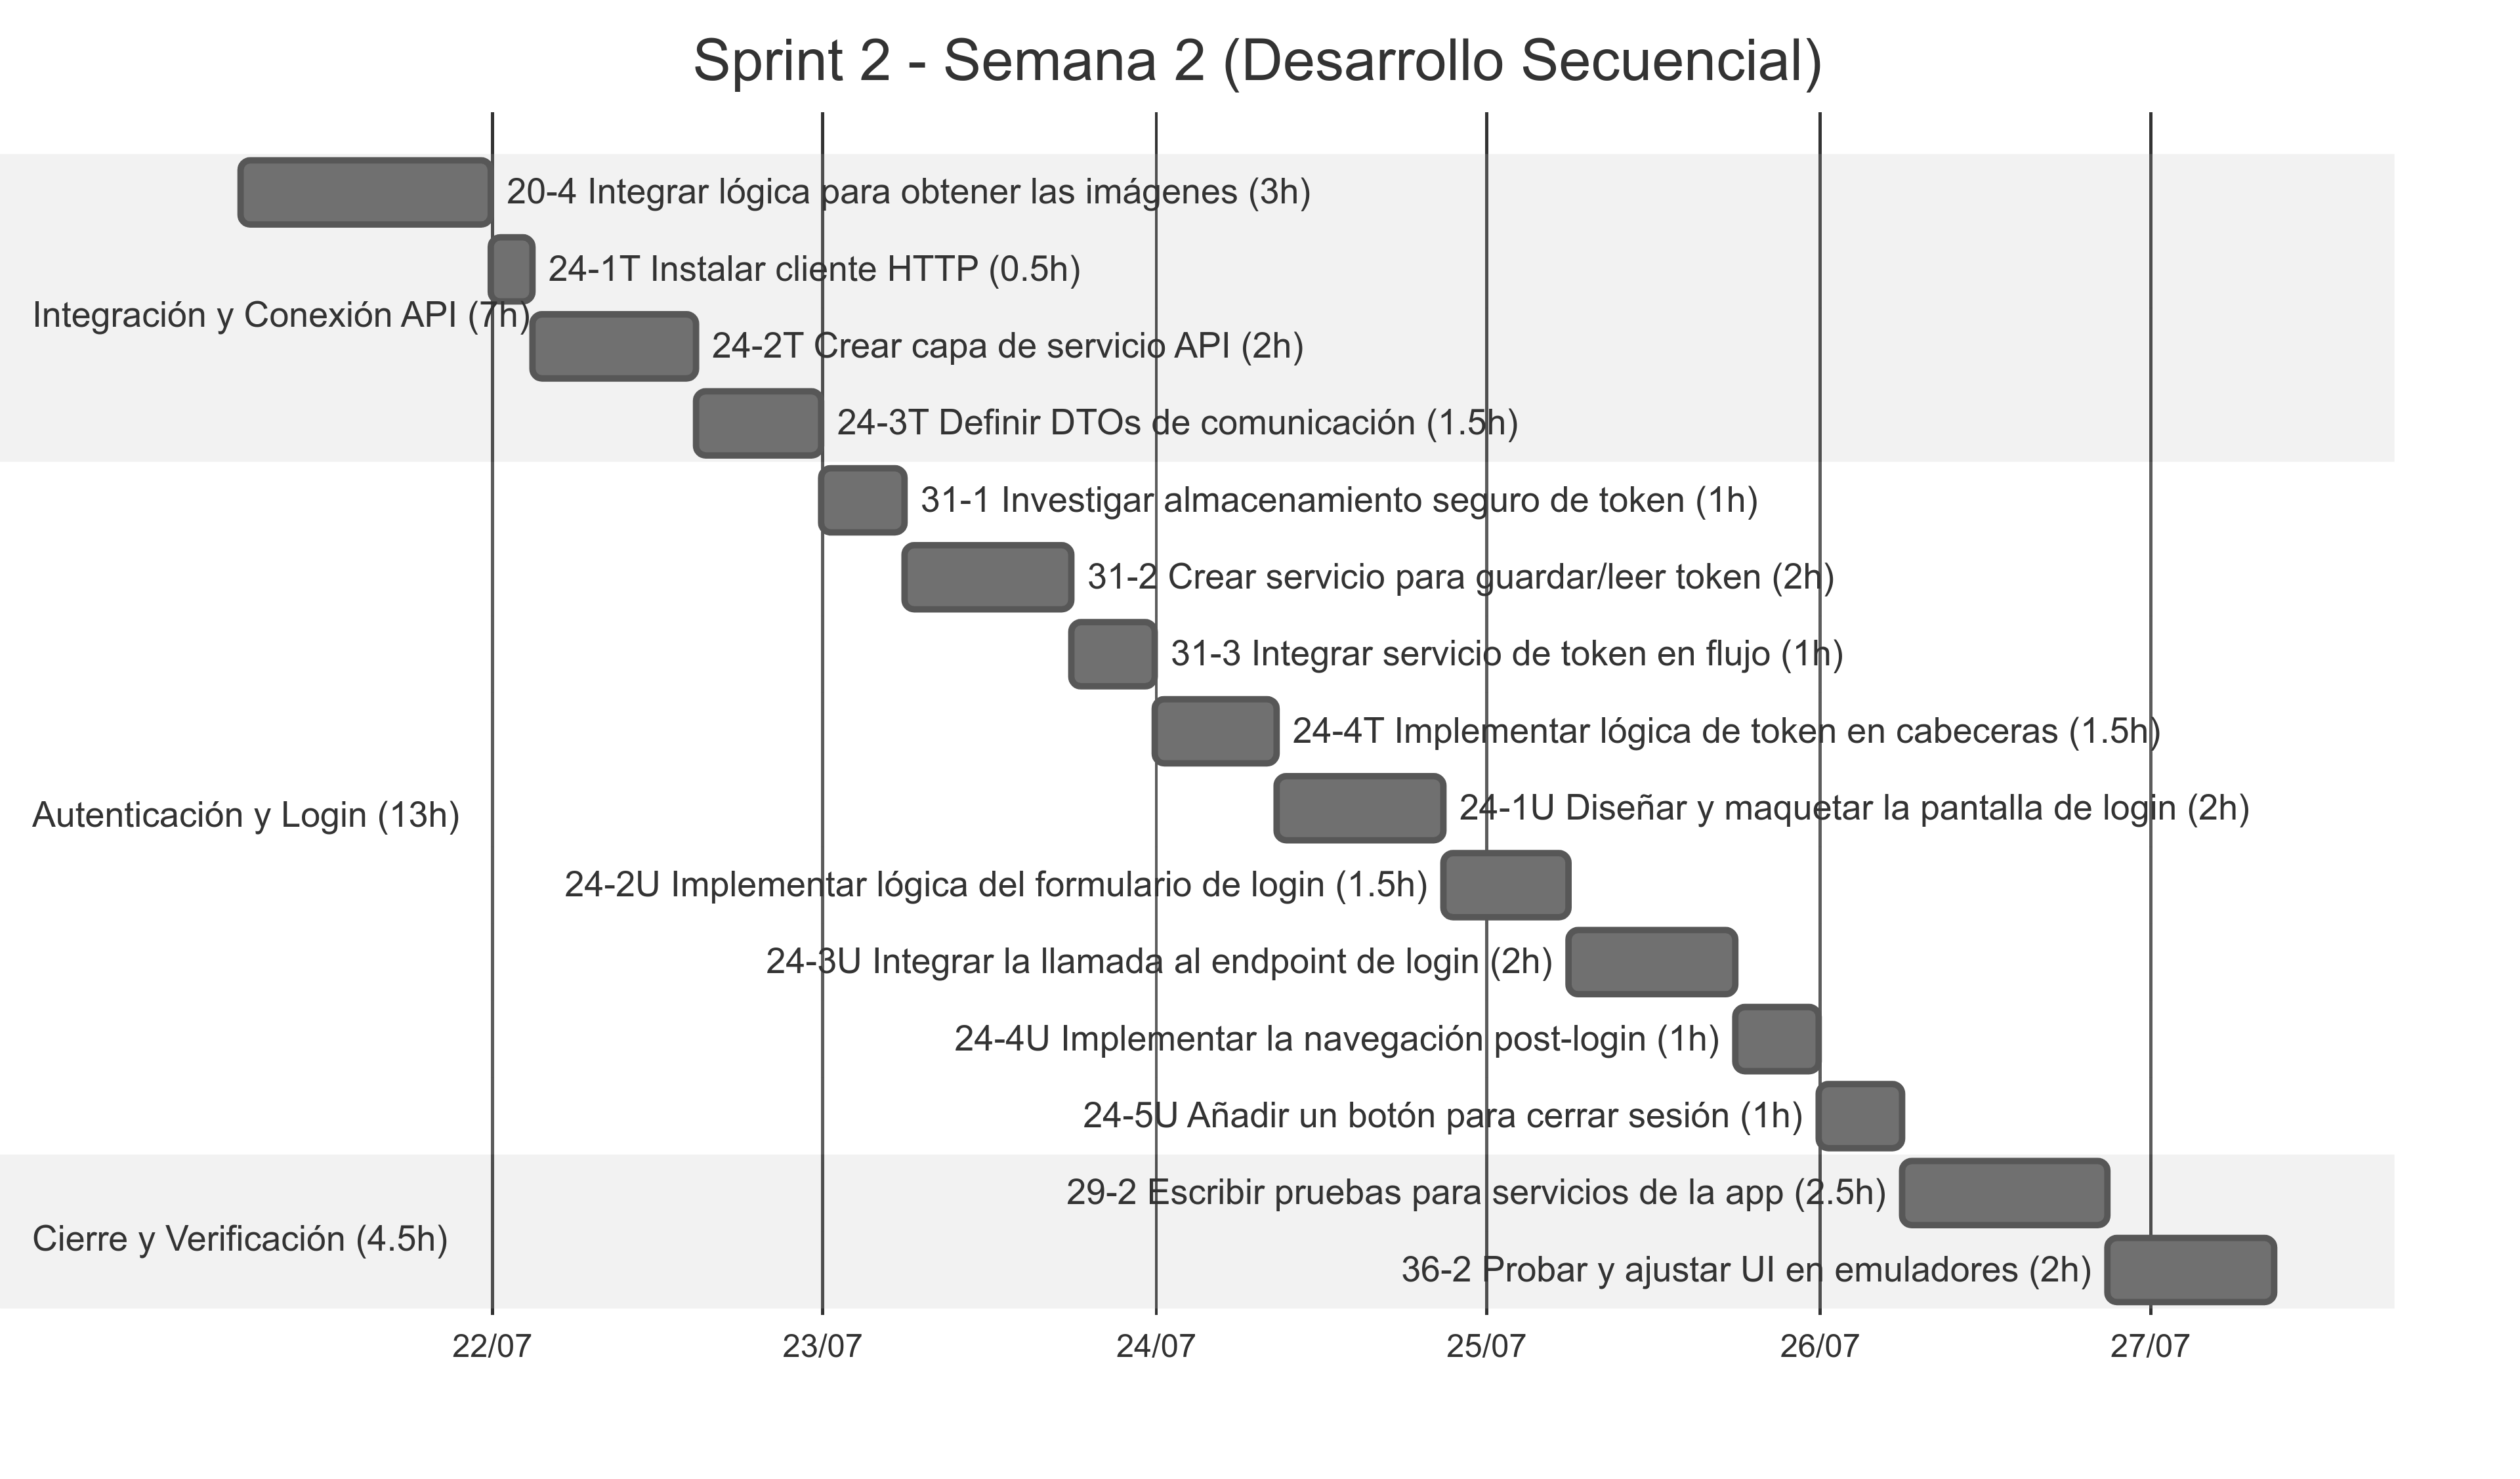
\includegraphics[width=0.8\textwidth]{assets/sprint2/week2-gantt.png}
    \end{center}
    \caption{Diagrama de Gantt de las tareas de la segunda semana del sprint 2}\label{fig:gantt-sprint2-week2}
\end{figure}


\subsection{Detalles de implementación}

\paragraph{Arquitectura del Cliente Móvil}
\subparagraph{}
Como se definió en la propuesta, la aplicación móvil seguirá los principios de la \textbf{Arquitectura Limpia}. Durante este sprint se materializará esta estructura creando los siguientes directorios y capas lógicas:
\begin{itemize}
    \item \textbf{Presentation}: Contendrá todos los componentes de React (Lynx.js), las pantallas (Login, Galería), y los hooks visuales. Es la capa más externa.
    \item \textbf{Domain}: Albergará las entidades de negocio (ej. `User', `MediaFile') y las definiciones de las interfaces de los repositorios (ej. `AuthRepository', `MediaRepository'). Esta capa no tendrá dependencias externas.
    \item \textbf{Application}: Contendrá los casos de uso (ej. `loginUser', `getLocalMediaFiles'). Orquestará el flujo de datos entre la `Presentation' y el `Domain', usando las interfaces de los repositorios.
    \item \textbf{Infrastructure}: Aquí residirán las implementaciones concretas de las interfaces del dominio. Se creará un `ApiAuthRepository' que use el cliente HTTP (HT24) y un `NativeMediaRepository' que use el módulo nativo implementado (HT23) para acceder a los ficheros del dispositivo.
\end{itemize}

\paragraph{Implementación de Módulos Nativos en Lynx.js}
\subparagraph{}
El reto técnico principal de este sprint es la creación de un módulo nativo para acceder a la galería (HT23). El proceso seguirá la documentación oficial de Lynx.js, que implica:
\begin{enumerate}
    \item Clonar y configurar el proyecto de `Lynx Explorer' para Android.
    \item En Android Studio, crear una nueva clase Java/Kotlin que herede de `LynxModule'.
    \item Dentro de esta clase, usar las APIs nativas de Android (`ContentResolver' y `MediaStore') para consultar las imágenes y vídeos del dispositivo. Este método también gestionará la solicitud de permisos (`READ\_MEDIA\_IMAGES').
    \item Exponer los métodos necesarios a JavaScript usando la anotación `@LynxMethod'.
    \item Registrar el módulo en la aplicación `Lynx Explorer'.
    \item Compilar una nueva versión del `Lynx Explorer.apk' que incluya nuestro módulo.
    \item Desde el código JavaScript de nuestra aplicación, podremos importar y llamar a este módulo para obtener los datos de la galería.
\end{enumerate}
Este proceso asegura un rendimiento nativo para una tarea intensiva como es el acceso a ficheros multimedia.
